\documentclass[12pt,a4paper]{article}
\usepackage{geometry}
\usepackage{graphicx}
\usepackage{amsmath}
\usepackage{amssymb}
\usepackage{array}
\usepackage{hyperref}
\usepackage{float}
\usepackage{listings}
\usepackage{caption}
\usepackage{subcaption}
\geometry{margin=1in}
\usepackage{tikz}
\usepackage{geometry}
\usetikzlibrary{positioning} 
\begin{document}

% Title Page
\begin{titlepage}
    \centering
    \begin{center}
        \includegraphics[width=0.5\textwidth]{logo.png} % Adjust width as necessary
    \end{center}
\begin{center}
    \textbf{Department of Computer Science and Engineering}\\
    Premier University
\end{center}
\begin{center}
    \textnormal{EEE 372 : Microprocessors \& Microcontrollers Laboratory}
\end{center}
    \huge
    \textbf{Project Proposal Report}\\
    \vspace{0.5in}
    \LARGE
    \textbf{Mobile Apps Controlled Smart Vehicle System}\\
    \vspace{1in}
    \large
    \textbf {Submitted by}\\
    \begin{center}
        \renewcommand{\arraystretch}{1.5} % Adjusts vertical spacing in the table
        \begin{tabular}{|>{\raggedright\arraybackslash}p{0.6\textwidth}|p{0.3\textwidth}|} % Adjust column widths
        \hline
        \textbf{Name} & \textbf{ID} \\
        \hline
        Mohammad Hafizur Rahman Sakib & 0222210005101118 \\
        \hline
        Arnab Shikder & 0222210005101098 \\
        \hline
        Shuvra Roy & 0222210005101093 \\
        \hline
        Sayed Hossain & 0222210005101102 \\
        \hline
        Mohammad Asmual Hoque Yousha & 0222210005101121 \\
        \hline
        \end{tabular}
        \end{center}
    \vspace{0.5in}
 
    \begin{minipage}[t]{0.5\textwidth}
        \textbf{Submitted to:}
        \\Nadim Bin Hossain
        \\Lecturer,Department of CSE
        \\ Premier University
        \\ Chittagong
    \end{minipage}%
    \begin{minipage}[t]{0.6\textwidth}
        \raggedleft
        \textbf{Remarks}\\
        \vspace{0.5cm} % Adjust vertical space for remarks
        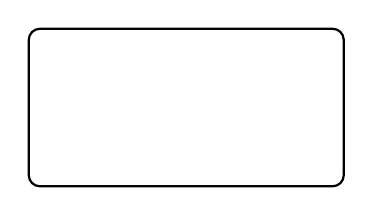
\begin{tikzpicture}
            \draw[thick, rounded corners] (0,0) rectangle (4,2);
        \end{tikzpicture}
    \end{minipage}

    \date{\today}
    \vfill
\end{titlepage}

% Abstract
\begin{abstract}
This proposal details the design and development of a Mobile Apps Controlled Smart Vehicle System using Arduino. The system enables users to control the vehicle's movement (left, right, forward, backward) via a mobile application. Additionally, the vehicle stops when an obstacle is detected in its path using ultrasonic sensors.
\end{abstract}

% Table of Contents
\tableofcontents
\newpage

% Introduction
\section{Introduction}
\label{sec:introduction}
This project proposes the development of a smart vehicle system that can be controlled via a mobile application. The vehicle will be capable of moving left, right, forward, and backward. It will automatically stop upon detecting obstacles using ultrasonic sensors, enhancing safety and usability.

% Objectives
\section{Objectives}
\label{sec:objectives}
The main objectives of this project are:
\begin{itemize}
    \item To develop a mobile application to control the vehicle’s movements.
    \item To integrate sensors for obstacle detection and automatic stopping.
    \item To design a user-friendly interface for the mobile application.
    \item To test and validate the system under various conditions.
\end{itemize}

% Methodology
\section{Methodology}
\label{sec:methodology}
\subsection{System Design}
The smart vehicle system will include an Arduino microcontroller, a Bluetooth module for communication, motor drivers for movement, and ultrasonic sensors for obstacle detection.

\begin{figure}[htbp]
    \centering
    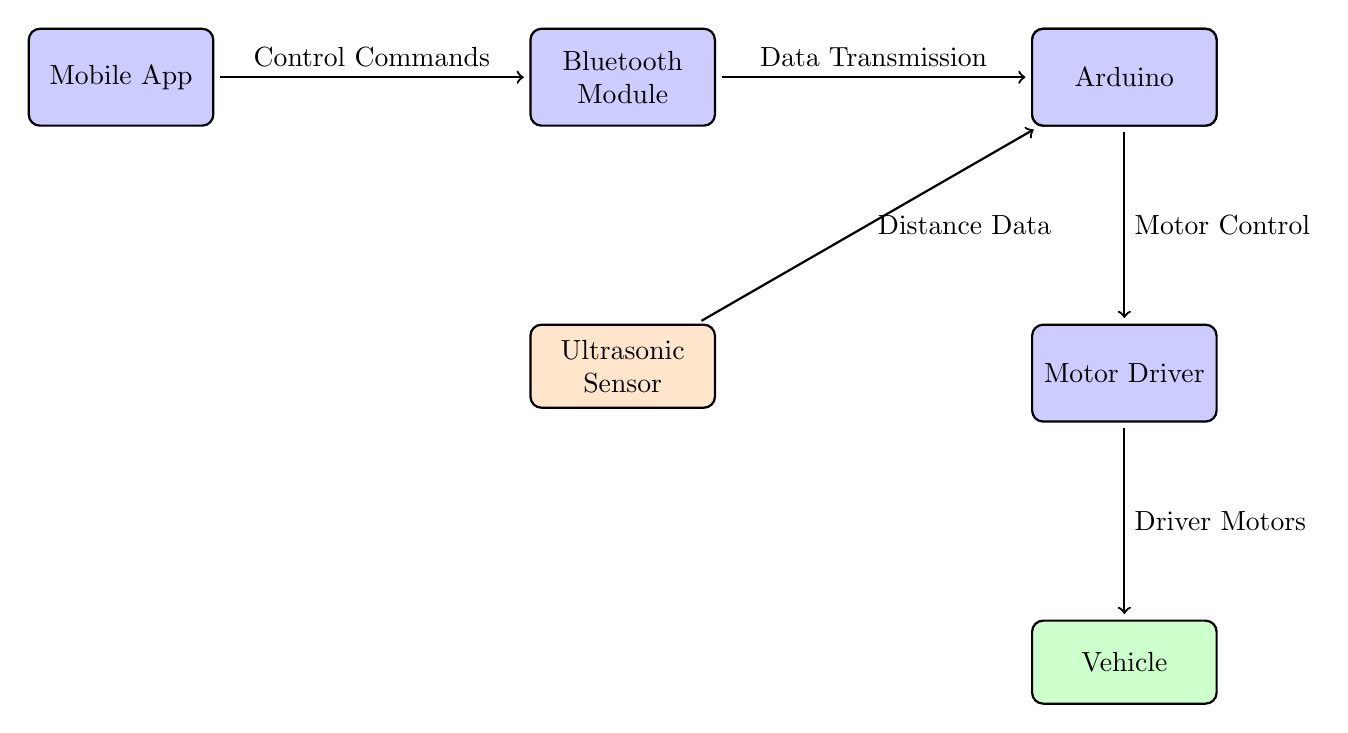
\begin{tikzpicture}[node distance=2.5cm and 2cm, auto, thick]

        % Styles
        \tikzstyle{block} = [draw, rectangle, rounded corners, minimum height=3.5em, minimum width=5em, text centered, text width=6em, fill=blue!20]
        \tikzstyle{sensor} = [draw, rectangle, rounded corners, minimum height=3em, minimum width=5em, text centered, text width=6em, fill=orange!20]
        \tikzstyle{vehicle} = [draw, rectangle, rounded corners, minimum height=3em, minimum width=5em, text centered, text width=6em, fill=green!20]
        \tikzstyle{arrow} = [->, thick, shorten <=2pt, shorten >=2pt]

        % Nodes
        \node [block] (mobile) {Mobile App};
        \node [block, right=4cm of mobile] (bluetooth) {Bluetooth Module};
        \node [block, right=4cm of bluetooth] (arduino) {Arduino};
        \node [block, right=4cm of bluetooth] (arduino) {Arduino};
        \node [block, below=of arduino] (motor) {Motor Driver};
        \node [sensor, below=of bluetooth] (sensor) {Ultrasonic Sensor};
        \node [vehicle, below=of motor] (vehicle) {Vehicle};

        % Arrows
        \draw[arrow] (mobile) -- node[above] {Control Commands} (bluetooth);
        \draw[arrow] (bluetooth) -- node[above] {Data Transmission} (arduino);
        \draw[arrow] (arduino) -- node[right] {Motor Control} (motor);
        \draw[arrow] (motor) -- node[right] {Driver Motors} (vehicle);
        \draw[arrow] (sensor) -- node[right] {Distance Data} (arduino);

\end{tikzpicture} 
\end{figure}

\begin{center}
    {\textbf{Figure 01 : Block Diagram of the Smart Vehicle System}}
\end{center}

\subsection{Hardware Components}
\begin{itemize}
    \item \textbf{Arduino Uno}: Acts as the main control unit for the vehicle.
    \item \textbf{HC-05 Bluetooth Module}: Enables communication between the mobile app and Arduino.
    \item \textbf{L298N Motor Driver}: Controls the motors to facilitate movement.
    \item \textbf{Ultrasonic Sensors}: Detects obstacles and triggers the vehicle to stop.
\end{itemize}

\subsection{Movement Control}
The vehicle will be capable of the following movements:
\begin{itemize}
    \item \textbf{Forward}: Move in the forward direction.
    \item \textbf{Backward}: Move in the backward direction.
    \item \textbf{Left}: Turn left.
    \item \textbf{Right}: Turn right.
    \item \textbf{Stop}: Halt when an obstacle is detected.
\end{itemize}

\subsection{Software Development}
The mobile application will be developed using Android Studio, chosen for its robust development environment and compatibility with Android devices. It will establish a Bluetooth connection with the vehicle to send control commands (e.g., left, right, up, down) to an Arduino microcontroller. The Arduino will be programmed using the Arduino IDE, integrating libraries for motor control and obstacle detection via an ultrasonic sensor. Additionally, a Java-based application sourced from a Youtube Video will be adapted to complement our project requirements, ensuring seamless integration with the smart vehicle system.

\subsection{Implementation Plan}
\begin{enumerate}
    \item \textbf{Design Phase}: Design the system architecture and select components.
    \item \textbf{Development Phase}: Develop the mobile app and Arduino code.
    \item \textbf{Integration Phase}: Integrate hardware and software components.
    \item \textbf{Testing Phase}: Test the system in different environments.
\end{enumerate}


% Expected Outcomes
\section{Expected Outcomes}
\label{sec:expected_outcomes}
The expected outcomes include:
\begin{itemize}
    \item A functional smart vehicle prototype.
    \item A mobile application to control vehicle movements.
    \item Successful integration of obstacle detection with automatic stopping.
    \item A detailed report on the design, development, and testing processes.
    \item A presentation about the project.
\end{itemize}

\section{Conclusion}

The Mobile Apps Controlled Smart Vehicle System successfully enables remote control of vehicle movements via a mobile application, facilitated by Arduino and Bluetooth technology. It incorporates real-time obstacle detection using ultrasonic sensors to ensure safe operation. Through meticulous hardware integration and software development using Android Studio and Arduino IDE, the system demonstrates robust functionality and usability. This project not only achieves its goals of creating a functional prototype but also highlights the practical application of embedded systems in modern transportation solutions. Future advancements could further optimize control algorithms and expand its application in robotics and smart vehicle technologies.

\end{document}
